\documentclass{IEEEtran}
\usepackage{amsmath}
\usepackage{parskip}
\usepackage{graphicx}
\usepackage{subfig}
% \usepackage[margin=1in]{geometry}

\newcommand{\bfu}{\mathbf{u}}
\newcommand{\bfv}{\mathbf{v}}
\newcommand{\bfx}{\mathbf{x}}
\newcommand{\bfy}{\mathbf{y}}
\newcommand{\bfpsi}{\mathbf{\psi}}
\newcommand{\bftheta}{\mathbf{\theta}}

\title{Tree-Structured Wavelet Compressive Sensing}

\author{David A. Neal and Josh Hunsaker}

\begin{document}
\maketitle

\begin{abstract}
Compressive sensing making use of wavelet transforms are commonly used
to help compress images as they are being captured.  Structure in
these transforms can be exploited and is commonly described by
zero-trees.  Convex optimization does not typically allow for
inclusion of this information, but Bayesian approaches allow for
priors to exploit structure.  Tree-structured wavelet compressive
sensing is presented as a new approach based on the introductory work
by He and Carin \cite{He09}.  This work presents a tutorial approach
to their work.  An attempt was made to impliment and
independantly verify the results, but was unsuccessful.  Performance
as reported in the original work is reported and the code generated
for the verification is included. 
\end{abstract}

\section{Introduction}

Many traditional sensor systems capture large amounts of data and then compress the data for transmission or storage purposes.  Compressive sensing provides an approach for combining the sensing and compressing stages into a single step.  This can provide both cost and efficiency benefits in sensor hardware. In the context of digital image processing, this can provide a way to capture a significantly reduced number of pixels while maintaining the ability to reconstruct the complete image later. Such reconstruction techniques require the use of a basis in which the image is sparse. One common approach is to use wavelet transforms as the basis for the image.

The wavelet transform of most natural images exhibits a ``zero tree''
structure in which the ``children'' of negligible coefficients tend to
be negligible as well. In \cite{He09}, the authors develop a
statistical algorithm which exploits the zero-tree phenomenon to
achieve increased reconstruction accuracy. By imposing a set of
Bayesian priors on the wavelet coefficients, the expected structure is
imposed statistically, which leads to a more flexible image model.

This paper reviews the theory behind the different elements of tree-structured wavelet
compressive sensing (TSW-CS) and how they fit together.  Starting with
wavelet transforms and moving through compressive sensing and
zero-trees, the paper concludes with an overview of Bayesian model and
expresses the algorithm described in \cite{He09} as a Gibbs sampling
model that itereratively estimates the original wavelet coefficients.

Results are reviewed from the original work.  An attempt to reproduce
the results was made, but was unsuccessful.  The paper concludes with
a discussion of what may have gone wrong.  The implemented code for
the algorithm is included as an appendix.

\section{Wavelet Transforms Of Natural Images}
\label{sec:wavelets}


\subsection{Discrete Wavelet Transform}

\begin{figure}[t]
  \centering
  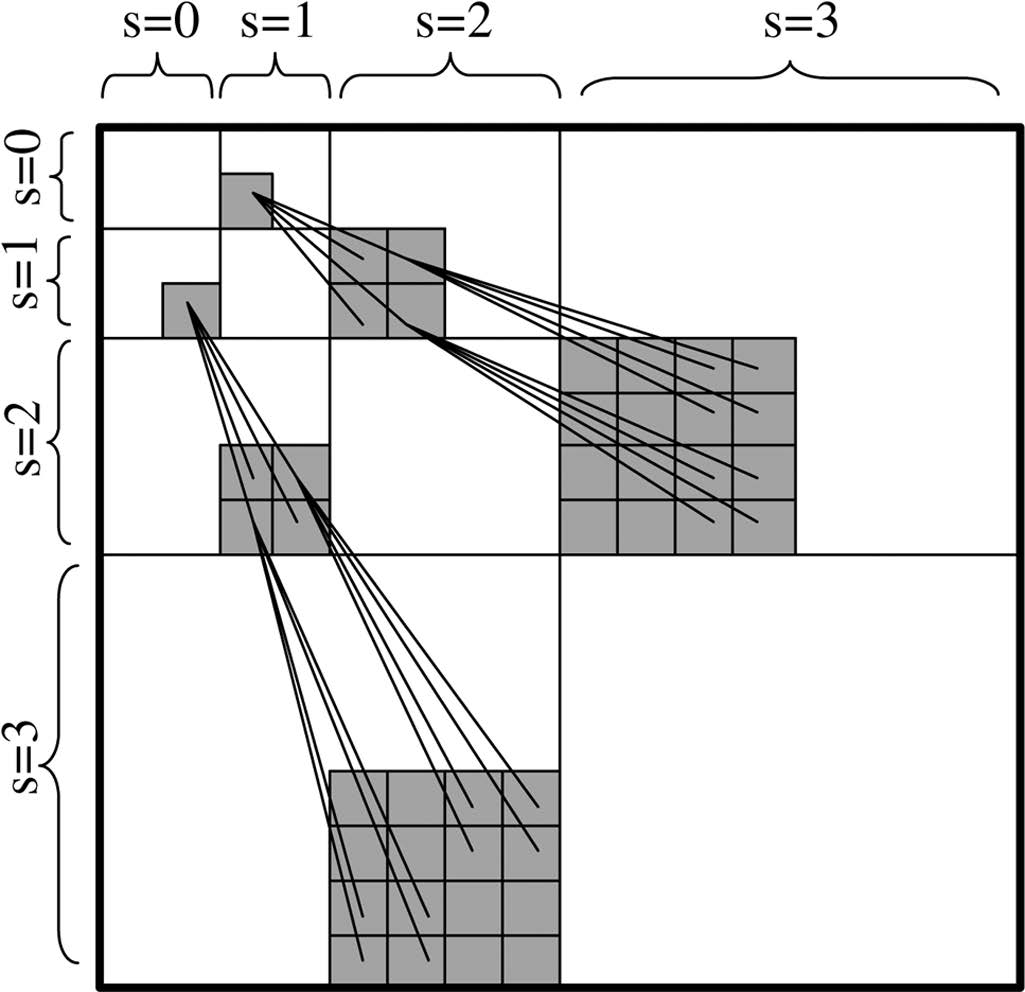
\includegraphics{wavelet_tree}
  \caption{Wavelet decomposition of an image, showing the tree structure. The top-left block
($s = 0$) represents scaling coefficients, and other regions are wavelet coefficients}
\label{fig:tree}
\end{figure}

A wavelet is a wave-like signal which has finite length. Wavelets are often used to model natural phenomena of finite duration.  While many wavelets are continuous and differentiable, we can also construct a class of wavelets which are discretely sampled for analysis of discrete signals.

Consider an orthogonal basis $\Psi$, whose columns $\bfpsi_j$ are discrete wavelets, we can decompose a signal $\bfx$ into a sum of wavelets as follows

\begin{equation}
  \label{eq:dwt}
  \bftheta = \Psi^T \bfx
\end{equation}

Each value $\theta_j$ represents the amount of the wavelet $\bfpsi_j$ present in $\bfx$. This is analogous to the discrete fourier transform, which breaks a signal into its component frequencies. Unlike the fourier transform however, wavelet transforms simultaneously capture both frequency and spacial information. Also, wavelet decompositions of natural signals tend to be sparse.  In other words, many natural signals can be constructed or approximated as the sum of a relatively small number of wavelets.

\subsection{Wavelet Tree Structure}
Discrete wavelet transforms of images have another property which may be exploited, which is the statistical relationship that exists between certain coefficients of the transform. The coefficients can be organized into a quadtree structure in which most coefficients serve as the parent for four other child coefficients. Within this structure, the coefficients which are the ``children'' of negligible coefficients will also be negligible with high probability.

Figure~\ref{fig:tree} shows an example of this tree structure in a transformed image.  The coefficients at scale $s=0$ serve as scaling coefficients for the coefficient trees, which each have their root node at scale $s=1$. The leaf nodes at the finest scale ($s=3$ in this example) represent the high-pass elements of the image.

\begin{figure*}[ht]
  \centering
  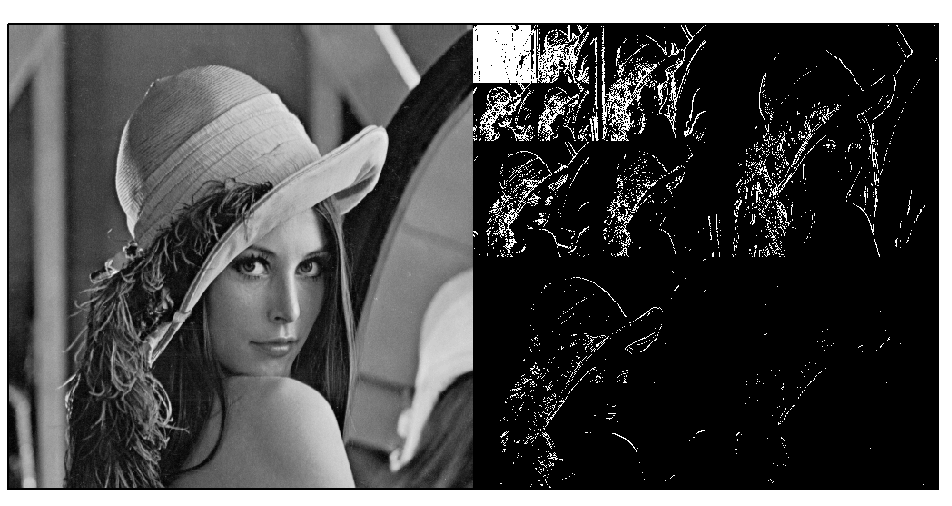
\includegraphics[width=0.8\textwidth]{lenna_wavelet}
  \caption{Example of multi-level wavelet transform. The original image is on the left, with the transformed image on the right.}
  \label{fig:lenna}
\end{figure*}

\section{Compressive Sensing}

\subsection{Sparse Signals}
Consider a discrete signal $\bfy$ of length $N$ in which all but $S$ of the values are zero. We say that $\bfy$ is ``$S$-sparse''.  Assume that we have prior knowledge about the sparsity of $\bfy$, but we do not have any specific information about \emph{which} of the samples are non-zero. If we sample $\bfy$ directly, we must take $N$ samples or we risk losing information.

Compressive sensing allows us to exploit the sparsity in $\bfy$ in order to collect less than $N$ data points.  In the absence of measurement noise we are able to reconstruct $\bfy$ perfectly, given sufficient data samples. Let $\Phi$ be a sensing matrix of size $M \times N$ with $M \ll N$. The following equation represents the compressive sampling operation:

\begin{equation}
  \label{eq:sense}
  \bfv = \Phi \bfy
\end{equation}

Now $\bfv$ is significantly smaller than $\bfy$ but should still contain enough information to reconstruct $\bfy$, as long as $\Phi$ is known. Of course, this depends upon $\bfy$ being sufficiently sparse, and upon $\Phi$ being chosen appropriately (which we will discuss in more detail in \ref{sub:incoherence}.)

We can also relax our definition of sparsity by considering any values that are sufficiently small to be insignificant.  Under this new definition, we will consider a signal to be $S$-sparse if all but $S$ of its values have a magnitude below some threshold $\epsilon$.  The signal is sparse in the sense that almost all of its energy is concentrated in a relatively small number of samples.  While such an assumption may lead to some error in the reconstruction, the energy in the error will be proportional to the energy in the negligible coefficients.

\subsection{Image Transform}

When working with image data, we have no guarantee of sparsity. In fact, for most interesting images the data will tend not to be sparse. This would seem to suggest that image data is not a good candidate for compressive sensing. However, as mentioned in section~\ref{sec:wavelets}, wavelets provide a basis in which most images have a sparse representation.  This means that if we had a way of sensing the wavelet coefficients instead of the pixel values, we would be sampling a sparse signal.

Consider a new sensing matrix
\begin{equation}
  \label{eq:newsense}
  \Phi^\prime = \Phi \Psi^T
\end{equation}

If we apply $\Phi^\prime$ to the image data $\bfx$, we get

\begin{equation}
  \label{eq:newsenseapplied}
  \begin{split}
  \bfv &= \Phi^\prime \bfx \\
  &= \Phi \Psi^T \bfx \\
  &= \Phi \bftheta
  \end{split}
\end{equation}

This means that sensing the image data with $\Phi^\prime$ is the same as sensing the (sparse) transform coefficients with $\Phi$.  Therefore, by using the measurements $\bfv$, we should be able to reconstruct the coefficient data and, by extension, the image.

\subsection{Incoherent Sampling}
\label{sub:incoherence}

It has been demonstrated \cite{Candes06b,Baraniuk06} that for compressive sensing of sparse signals, taking random measurements is in some sense an optimal strategy. For example, the rows of the sensing matrix $\Phi$ may be a collection random test vectors ${\phi_k}$ such as gaussian white noise or a series of bernoulli random variables.

Under such a sensing scheme, the number of samples required will be inversely proportional to the similarity between the sensing modality ($\Phi$) and the signal model ($\Psi$).  We can estimate this similarity by measuring the mutual coherence $\mu(\cdot)$ as follows \cite{Donoho01,Candes06}

\begin{equation}
  \label{eq:coherence}
  \mu(\Phi \Psi) = \underset{k,j}{max}| \langle \phi_k, \psi_j \rangle | .
\end{equation}

In the implementation of this project, we have constructed the rows of $\Phi$ as a series of bernoulli random variables.  We found the mutual coherence between our sensing matrix and our wavelet basis to be around 2.75.  While it is possible to construct a sensing matrix whose coherence with the wavelet basis is ideal ($\mu(\Phi \Psi)=1$), such matrices are almost always complex-valued which would significantly complicate the algorithm being used.

\subsection{Reconstruction}

The most straightforward way to reconstruct a sparse signal from compressed samples is via an $\ell_1$ minimization known as \emph{basis pursuit}.  By solving the simple convex optimization problem

\begin{equation}
  \label{eq:bp}
  \bftheta = \underset{\tilde\bftheta}{\arg \min}\; \|\tilde\bftheta\|_{\ell_1}\; \text{s.t.} \; \bfv = \Psi \tilde\bftheta ,
\end{equation}

we acquire the coefficient vector $\bftheta$ with minimum $\ell_1$ norm which satisfies the measurement data.  Since the $\ell_1$ norm emphasizes sparsity, we are essentially solving for the sparsest vector that can explain the data.

\section{Bayesian Inference}

In a maximum likelihood sense, the goal is to use the samples
$\mathbf{v}$ to estimate the most likely $\mathbf{\theta}$.  If $p(\mathbf{\theta}|\mathbf{v})$ is known, then the
maximum likelihood value of $\mathbf{\theta}|\mathbf{v}$ can be
found.  As in many cases, this density is not known.  The most common
approach is to apply Bayes' theorem, which yields
$p(\mathbf{v}|\mathbf{\theta})p(\mathbf{\theta})/p(\mathbf{v})$.  In
  this case, these densities are also not known, but some things are
  known about them.

If a density is selected based on what is known , the parameters are
still unknown.  However, in this case, the problem can be stated as
$p(\mathbf{\theta},\mathbf{\xi}|\mathbf{v})$, with $\mathbf{\xi}$
representing a vector of all the density parameters that are not
known.  Again applying Bayes' theorem, the problem becomes
$p(\mathbf{v}|\mathbf{\xi},\mathbf{\theta})p(\mathbf{\theta},\mathbf{\xi})/p(\mathbf{v}|\mathbf{\xi})$.
As in many problems, the denominator is simply a scaling constant and
does not affect the choice of $\mathbf{\theta}$ and $\mathbf{\xi}$
that maximize the likelihood.  

Conditionally factoring the result and splitting up $\mathbf{\xi}$
into the different parameters yields

\begin{equation}
p(\mathbf{v}|\mathbf{\alpha}_n,\mathbf{\theta})p(\mathbf{\theta}|\mathbf{\mu},\mathbf{\pi},\mathbf{\alpha}_s)p(\mathbf{\alpha}_s)p(\mathbf{\alpha}_n)p(\mathbf{\pi})p(\mathbf{\mu}).
\label{bayesprimary}
\end{equation}

In \cite{He09}, they assume that
$p(\mathbf{v}|\mathbf{\alpha}_n,\mathbf{\theta})$ is distributed Gaussin,
so $\mathbf{\alpha}_n$ is the precision and the mean $\phi
\mathbf{\theta}$.  The mean is based on (\ref{eq:sense}) and the
precision is based on the noise in the measurement, which is
Gaussian.  They assume that $\mathbf{\theta}$ is a spike
and slab distribution, which means that some percentage of the time
outcome is zero and the rest of the time it is a Gaussian draw.  For this distribution,
$\mathbf{pi}$ represents the probability that the Gaussian draw is
chosen, $\mathbf{\mu}$ is the mean of that Gaussian, and
$\mathbf{\alpha}_s$ is the precision.  This is based on the fact that
$\mathbf{\theta}$ is sparse, so there are many zeros or small
coefficients, and the rest of the coefficients are assumed to be
Gaussian based around different means and variances common to their
scale in the transform (hence the subscript $s$ on
$\mathbf{\alpha}_s$).

One issue remains to be able to solve this problem.  The distributions of the
parameters must be determined.  A common distribution for precision
parameters is the Gamma distribution.  This is a common choice due to
it being a conjugate distribution to a Gaussian distribution.  This
means that when it is used as a prior to the Gaussian, as with Bayes'
theorem, the result is still a Gaussian distribution.  This is
desirable because it makes solving the problem somewhat easier. 

The distribution on $\mathbf{\pi}$ is set to a Beta distribution.  This
works well because the two parameters of the Beta distribution can be
set to pick between them with one providing numbers closer to one and
the other providing numbers closer to zero.  This can be used to
weight the choice in the spike and slab distribution between the zero
and the Gaussian.  

There are means for estimating all the parameters and solving for the
maximum likelihood solution.  This typically involves some
significantly difficult math.  In many cases, it is desirable to solve
the problem directly, but given that for a $128\times128$ image, there
are $128^2$ elements in many of the vectors, the problem complexity is
high.  An alternative approach that is typically applied is Gibbs
sampling.

\subsection{Gibbs Sampling}

Gibbs sampling is an approach for determining a density by sampling
from it.  If a problem is set up similar to how (\ref{bayesprimary})
has been found, random draws for each parameter can be used
flowed to estimate average paramaters and allow for draws from the primary distributions.  In this
case, the lower level parameter distributions are able to exploit information
about structure or values and are considered prior distributions.
Exploiting this prior information is one of the main benefits to selecting a Bayesian approach over
convex optimization approaches.  

The random draws can be run for a period of time with each iteration
updating the estimation of the top level parameters. After a burn in
period, it has been shown that this
converges to the true distribution \cite{Mackay03}.  Since the true
distribution of $\mathbf{\theta}$ given its parameters has been determined, a series of random samples can be drawn
and the maximum likelihood value can be estimated from the
distribution.

\subsection{Implemented Gibbs Sampling}

In order to implement the Gibbs sampling approach for this model, the
actual prior probabilities for the parameters had to be
determined. Each parameter makes use of the prior information
available to it and the structure that the model is imposing on it.

The first thing to consider is the structure of the model.  The
goal is to find $\mathbf{\theta}$, but the structure of the wavelet
transform needs to be exploited.  Since the structure of the wavelet
transform changes with the scale, it is important to consider the
scale of each element of $\mathbf{\theta}$.  As such, the model bases
all of the parameters on the scale.  They also look at each element of
each scale individually.  

\begin{figure}[ht]
  \centering
  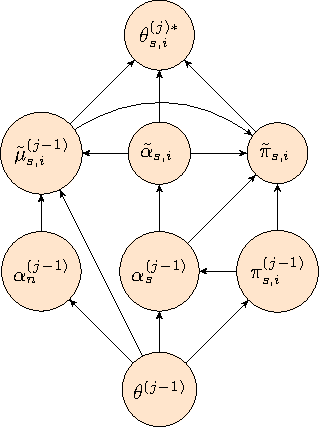
\includegraphics[width=1\linewidth]{bayes_graph}
  \caption{Simplified Graph of the Bayesian Model}
  \label{bayesfun}
\end{figure}

A graphical approach is often used to show the interrelationships
between the different elements in a Bayesian model.  Figure
\ref{bayesfun} shows a graph of the major elements that are either
calculated or randomly drawn.  All other coefficients are fixed and
feed into the appropriate lower level elements.  The
equations for drawing or calculating these values given below express
these interrelationships.


The data is used to help determine the noise precision
$\mathbf{alpha}_n$.  Since this noise is due to things like
measurement noise, it does not change with scale or element, so there
is only one value.  The distribution is given as 
\begin{equation}
 p(\alpha_n^{(j)}|-) =
    \Gamma(a_0+N/2,b_0+\|(\mathbf{v}-\phi\mathbf{\theta}^{(j)})\|/2 .
\label{alphan}
\end{equation}
The Gamma distribution has a $a_0$ and $b_0$ as $10^{-6}$ to keep the
arguments away from zero.  The $N$ value is the number of elements in
$\mathbf{\theta}$, while the vectpr-matrix value in the second
parameter is the mean-square error divided by two.  When the error is
small, the large number for the first parameter means that values of
$\mathbf{alpha}_n$ will most likely be large.  This makes sense, since
the estimate is close and the noise is probably small.  As the error
increases in size, the estimate of the noise is more likely to be
large, but is still evenly balanced with potentially small values.
This both exploits information from the data $\mathbf{v}$ and changes
its value based on the amount of error in the current estimation.

For the estimation of $\mathbf{\alpha}_s$, the $s$ subscript indicates
that the value is changing at each scale.  The distribution is given
as 
\begin{equation}
    p(\alpha_s^{(j)}|-) =  \Gamma(c_0+0.5\sum_{i=1}^{M_s}\mathbf{1}(\theta_{s,i}^{(j)}\neq
    0), d_0+0.5\sum_{i=1}^{M_s}\theta_{s,i}^{2,(j)})).
\label{alphas}
\end{equation}
Again, the values of $c_0$ and $d_0$ are set to $10^{-6}$.  The value
of $M_s$ is the number of elements at scale $s$.  The
$\mathbf{1}(x)$ is zero if $x$ is false and one if $x$ is true.  So
the first argument is counting the number of non-zero elements in
$\mathbf{\theta}$ at scale $s$ and element number $i$ and the
second is counting the squared magnitude of those elements.  This
means that when the values are small, the precision will tend to be
large, but when the elements are large, the precision can be smaller.
This allows for variation across the elements relative to their
magnitude.

The final parameter to draw for is $\mathbf{\pi}$.  This parameter
determines the probabilility of an element being from the zero
distribution or the Gaussian distribution when drawing for
$\mathbf{\theta}$.  The scale zero elements are typically non-zero, as
these are scaling elements for the entire image, so those elements are
set to $1$.  These probabilities are also related to the parent-child
relationships in the transform, so they change with scale.
Additionally, the scale $1$ elements have no parents.  This results in
the distribution for $s=1$ being given as
\begin{equation}
    p(\pi_r^{(j)}|-)  = 
    \beta(e_0^r+\sum_{i=1}^{M_s}\mathbf{1}(\theta_{s,i}^{(j)}\neq
    0), f_0^r +\sum_{i=1}^{M_s}\mathbf{1}(\theta_{s,i}^{(j)}= 0)).
\label{pir}
\end{equation}
Here, $e_0^r = .9M_s$ and $f_0^r = .1M_s$.  The two indicator functions compare the number of elements that are
non-zero for the first argument and that are zero for the second.
When the first argument is larger, the Beta distribution selects a probability tends toward $1$
and when the second is, it tends toward $0$.  This effectively selects
a probability based on the current estimate of $\mathbf{\theta}$.

For scales larger than $1$, there are two distributions.  The first is
\begin{equation}
  \begin{array}{ccc}
    p(\pi_s^{0,(j)}|-) & = &
    \beta(e_s^{s0}+\sum_{i=1}^{M_s}\mathbf{1}(\theta_{s,i}^{(j)}\neq
    0,\theta_{pa(s,i)}^{(j)}= 0), \\
    & & f_s^{s0} +\sum_{i=1}^{M_s}\mathbf{1}(\theta_{s,i}^{(j)}=
    0,\theta_{pa(s,i)}^{(j)}= 0)),
  \end{array}
\label{pir0}
\end{equation}
which draws for the case where the parent of the $s,i$th element is
zero and the other is
\begin{equation}
  \begin{array}{ccc}
    p(\pi_s^{(1,j)}|-) & = & 
    \beta(e_s^{s1}+\sum_{i=1}^{M_s}\mathbf{1}(\theta_{s,i}^{(j)}\neq
    0,\theta_{pa(s,i)}^{1,(j)}\neq 0), \\
    & & f_s^{s1}+\sum_{i=1}^{M_s}\mathbf{1}(\theta_{s,i}^{(j)}=
    0,\theta_{pa(s,i)}^{(j)}\neq 0)),
  \end{array}
\label{pi0}
\end{equation}
which draws for the case where the parent is non-zero.  In these
equations, $e_0^{s0} = M_s/N$, $f_0^{s0} = (1-1/N)M_s$, $e_0^{s1} =
.5M_s$, and $f_0^{s1} = .5M_s$. Again, the
balance in the equation is set to draw a probability based on the what
the number of zero versus non-zero elements suggests.  Then, for each
$s,i$, the value for $\pi_{s,i}$ is selected from these two by
\begin{equation}
  \begin{array}{ccc}
     
    & & \\
    \pi_{s,i}^{(j)} &= & \left\{ 
    \begin{array}{ccc}
      %\pi_{sc} & if & s= 0 \\
     % \pi_r^{(j)} & if & s = 1  \\ 
      \pi_s^{0,(j)} & if & 2 \leq s \leq L, \theta_{pa(s,i)} = 0  \\ 
      \pi_s^{1,(j)} & if & 2 \leq s \leq L, \theta_{pa(s,i)} \neq= 0 
    \end{array} \right. \\
  \end{array}
\label{pichoose}
\end{equation}

Now, in order to draw for each $\theta_{s,i}$, the value for the mean,
precision, and $\pi$ must be estimated for that specific element.
This can be determined by taking an expected value for the theta with
respect to the specific elements.  The result is

\begin{equation}
    \tilde{\alpha}_{s,i} = \alpha_s + \alpha_n
    \mathbf{\phi}_m^T\mathbf{\phi}_m,
\label{alphatilde}
\end{equation}
\begin{equation}
    \tilde{\mu}_{s,i} = 
    \tilde{\alpha}_{s,i}^{-1}\alpha_n\mathbf{\phi}_m^T(\mathbf{v}-\sum_{k=1,k\neq
      m}^N\mathbf{\phi}_k\theta_k)
\label{mutilde}
\end{equation}
\begin{equation}
  \begin{array}{cc}
    \tilde{\pi}_{s,i}   =  1, s = 0\\
    \frac{\tilde{\pi}_{s,i}}{1-\tilde{\pi}_{s,i}}  =
    \frac{\pi_{s,i}}{1-\pi_{s,i}}\frac{\mathcal{N}(0,\alpha_s^{-1})}{\mathcal{N}(\tilde{\mu}_{s,i},\tilde{\alpha}_{s,i}^{-1})},
    &1 \leq s \leq L.
  \end{array}
\label{pitilde}
\end{equation}
Here, $\mathbf{\phi}_m$ is the $m$th column of $\phi$ and $\theta_k$ is
the $k$th element of $\mathbf{\theta}$.  

These estimations of the
parameters of $\theta_{s,i}$ can then be used to draw from 
\begin{equation}
    p(\theta_{s,i}|-)  = 
    (1-\tilde{\pi}_{s,i})\delta_0+\tilde{\pi}_{s,i}\mathcal{N}(\tilde{\mu}_{s,i},\tilde{\alpha}_{s,i}^{-1}),
\label{thetatilde}
\end{equation}

\section{Algorithm}

The actual algorithm for the model is not calculated in the order
given above, as the updates and draws occur relative to a sample of
$\mathbf{\theta}$.  The algorithm is run by initializing a value for
each $\theta_{s,i}$.  This is then used to initialize the random draws
in (\ref{alphan}-\ref{pichoose}).  These values are then used with the
initial $\theta_{s,i}$ to initialize the estimates for
(\ref{alphatilde}-\ref{pitilde}).

Once this initialization takes place, the algorithm loops by drawing a
new set of $\theta_{s,i}$ from (\ref{thetatilde}), updating the
estimates for the parameters in (\ref{alphatilde}-\ref{pitilde}), and
then drawing new values from (\ref{alphan}-\ref{pichoose}).

In the paper, they found that this converges to the true distribution
in about $200$ iterations.  After this, they found that $100$ samples
was sufficient to estimate $\mathbf{\theta}$ accurately.

In the paper, they note that this can be drawn sequentially by drawing
for each $(s,i)$ and then incorporating it into the draw for $(s,i+1)$.  It can also be drawin
in a block method, drawing all the $\theta_{s,i}$ at once.  Drawing
sequentially converges faster since the newer data is better and is
incorporated earlier into the updates.

\section{Results}

In this paper, the algorithm proposed was compared with seven recently
developed algorithms.  The mean and variance for each algorithm was
calculated and the algorithm was run in Matlab.  All examples used
$128\times128$ images and set scale zero as an $8\times8$.  The
calculated relative reconstruction error was found by
$||\mathbf{x}-\hat{\mathbf{x}}\\_2/||\mathbf{x}||_2$, where
    $\mathbf{x}$ is the original image and $\hat{\mathbf{x}}$ is the
recovered image.  The images used were natural images from Microsoft
Research and are available at http://research.microsoft.com/en-us/projects/objectclassrecognition/.
Several plots and tables taken from the original article are presented
and discussed here as a summary of the algorithm performance.

The results show that the algorithm outperforms all the algorithms
with which it was compared in the sense that the mean and standard
deviation are smaller for $2000$ and $6000$ samples, as seen in
Figures \ref{table1} and \ref{table2}.

\begin{figure}[ht]
  \centering
  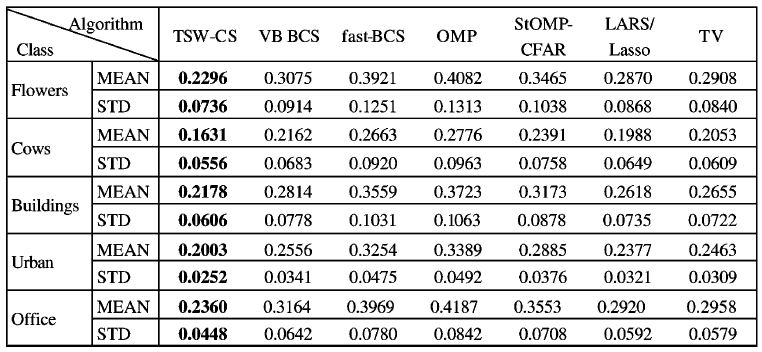
\includegraphics[width=1\linewidth]{he_carin_results_m2000}
  \caption{Results from He and Carin paper for $2000$ samples}
  \label{table1}
\end{figure}

\begin{figure}[ht]
  \centering
  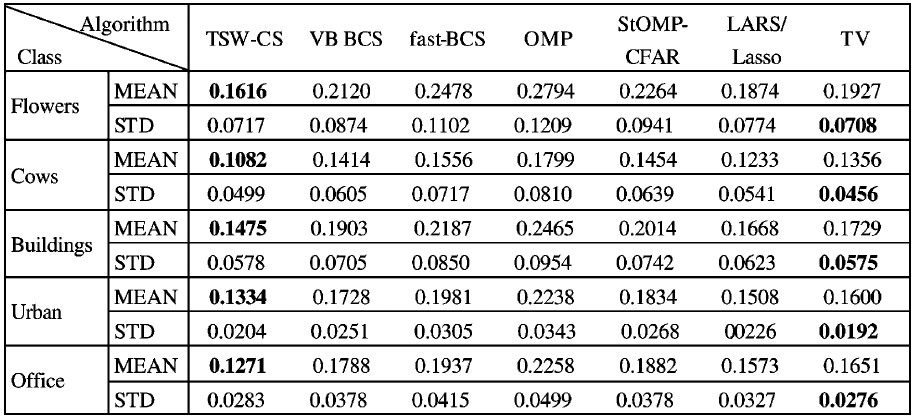
\includegraphics[width=1\linewidth]{he_carin_results_m6000}
  \caption{Results from He and Carin paper for $6000$ samples}
  \label{table2}
\end{figure}


Figure \ref{accplot}  shows that the
relative reconstruction error is smaller over all tested numbers of
measurements. 
 
\begin{figure}[ht]
  \centering
  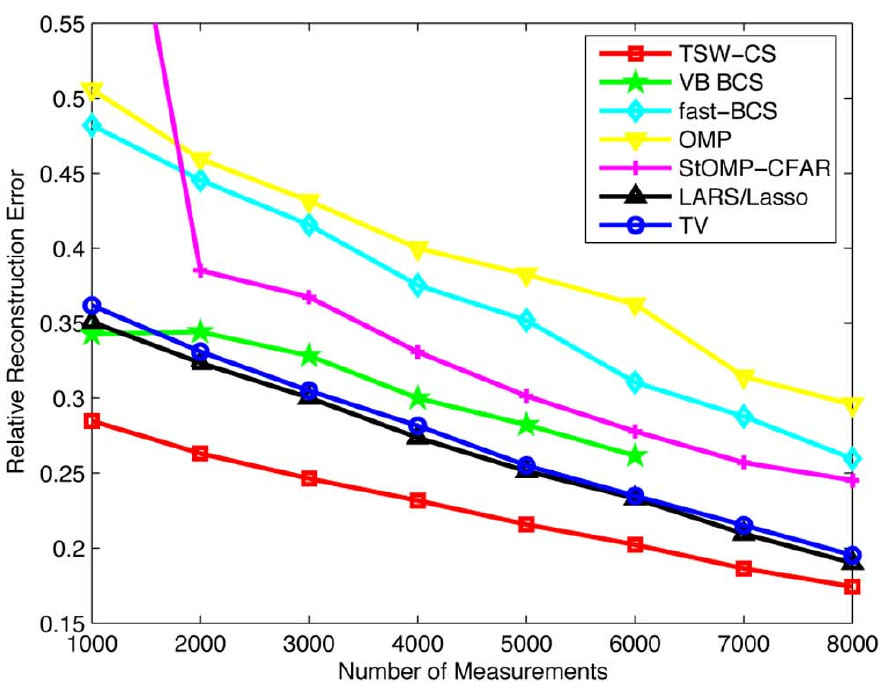
\includegraphics[width=1\linewidth]{he_carin_merror_plot}
  \caption{Measurement Error versus Number of Measurements from He and Carin paper}
  \label{accplot}
\end{figure}

Figure \ref{cputime} shows the amount of time that each algorithm ran.  It is
most interesting that the speed did not appreciably decrease when more
samples were drawn, while most of the other algorithms appear to
slow down significantly as the number of samples increases.

\begin{figure}[ht]
  \centering
  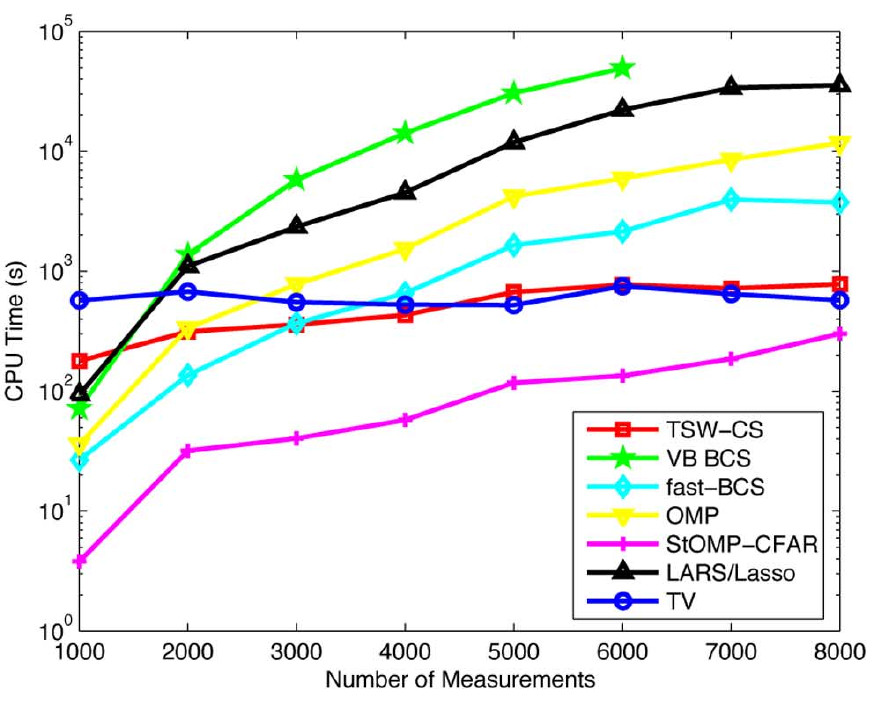
\includegraphics[width=1\linewidth]{he_carin_speed}
  \caption{Algorithm CPU Time versus Number of Measurements from He and Carin paper}
  \label{cputime}
\end{figure}

Comparison of the estimated wavelet coefficients provides some
insight.  Figure \ref{wave1} shows the coefficients with $2000$
samples.  The red is the true values.  Most of the estimators have
many non-zero large coefficients as the coefficient index increases,
while only TSW-CS has set them to zero.  While this introduces error
by ignoring some significant coefficients, Figure \ref{wave2} shows
the superior matching for the earlier coefficients.  Between this and
the large magnitude of the estimates at higher indicies for other
algorithms, the smaller error is easy to understand.

\begin{figure}[ht]
  \centering
  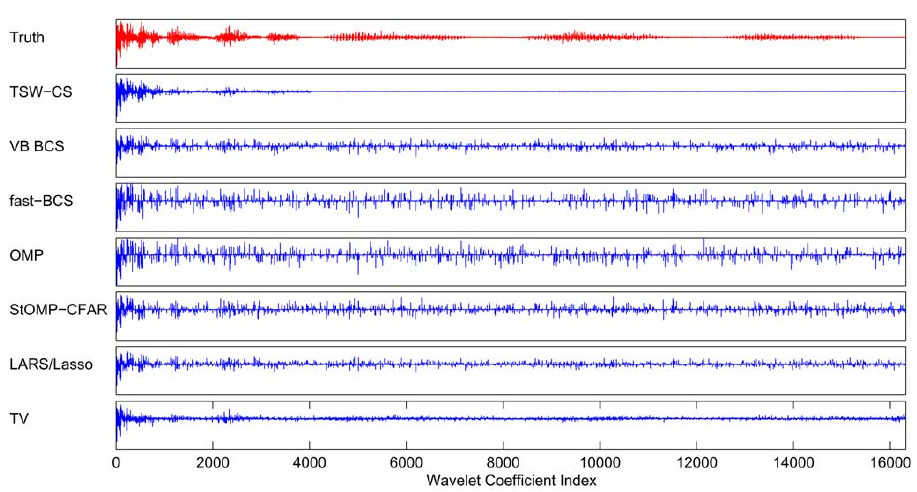
\includegraphics[width=1\linewidth]{he_carin_wavelet_whole}
  \caption{Comparison of All Wavelet Coefficients for each Algorithm
    with $2000$ Measurements}
  \label{wave1}
\end{figure}

\begin{figure}[ht]
  \centering
  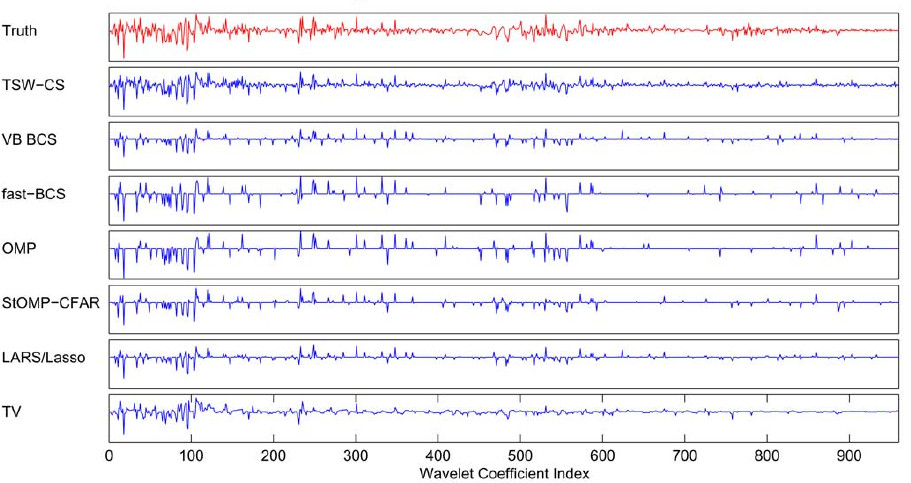
\includegraphics[width=1\linewidth]{he_carin_wavelet_s1and2}
  \caption{Comparison of Scale 1 and 2 Wavelet Coefficients for each Algorithm with $2000$ Measurements}
  \label{wave2}
\end{figure}

When the number of measurments is increased to $6000$, the match is
even better, as shown in Figure \ref{wave3}.  The algorithm starts to
pick up the significant values at the higher indicies as well.  This
is also more apparent in other algorithms.

\begin{figure}[ht]
  \centering
  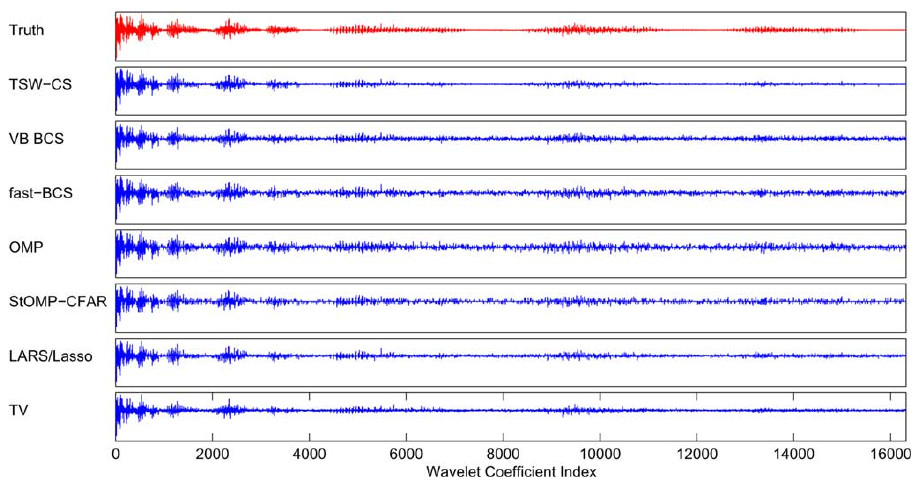
\includegraphics[width=1\linewidth]{he_carin_wavelet_6000}
  \caption{Comparison of All Wavelet Coefficients for each Algorithm
    with $6000$ Measurements}
  \label{wave3}
\end{figure}

In order to emphasize the improvement with more samples, Figure
\ref{wave4} shows the error bars on just the first $50$ estimated
coefficients.  As can be seen, the error bars decrease significantly
as the number of measurements goes up.

\begin{figure}[ht]
  \centering
  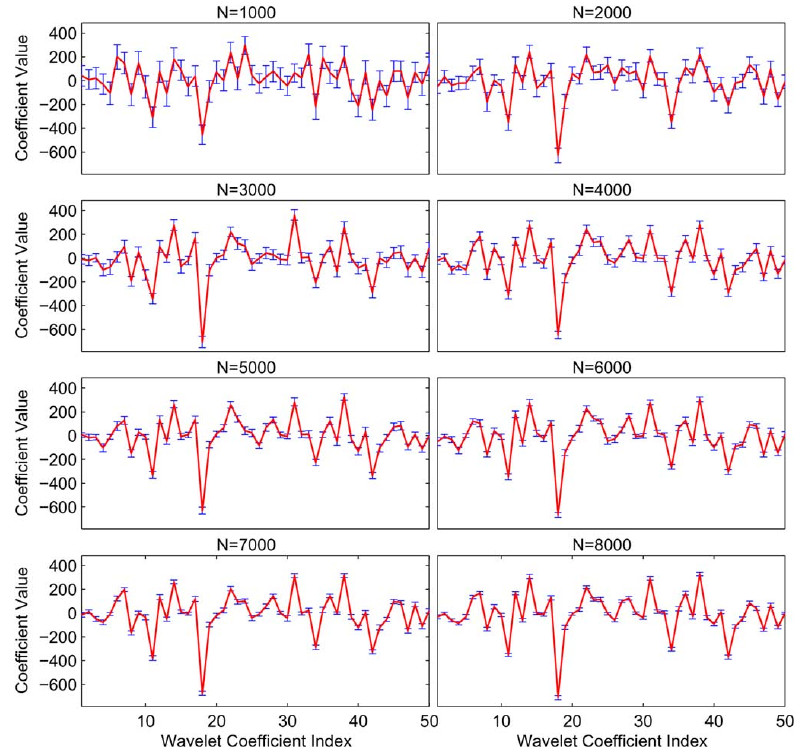
\includegraphics[width=1\linewidth]{he_carin_errorbars}
  \caption{Error Bars for the first $50$ coefficients with various
    numbers of measurements}
  \label{wave4}
\end{figure}

Figure~\ref{fig:bp-results} shows the result of six trials of the basis pursuit algorithm to construct an image from 2000 samples.  Sampling at this rate represents a compression ratio of 8:1. While the images appear somewhat blurry, their relative error is fairly small.

\begin{figure*}[ht]
  \centering
  \subfloat[][]{%
    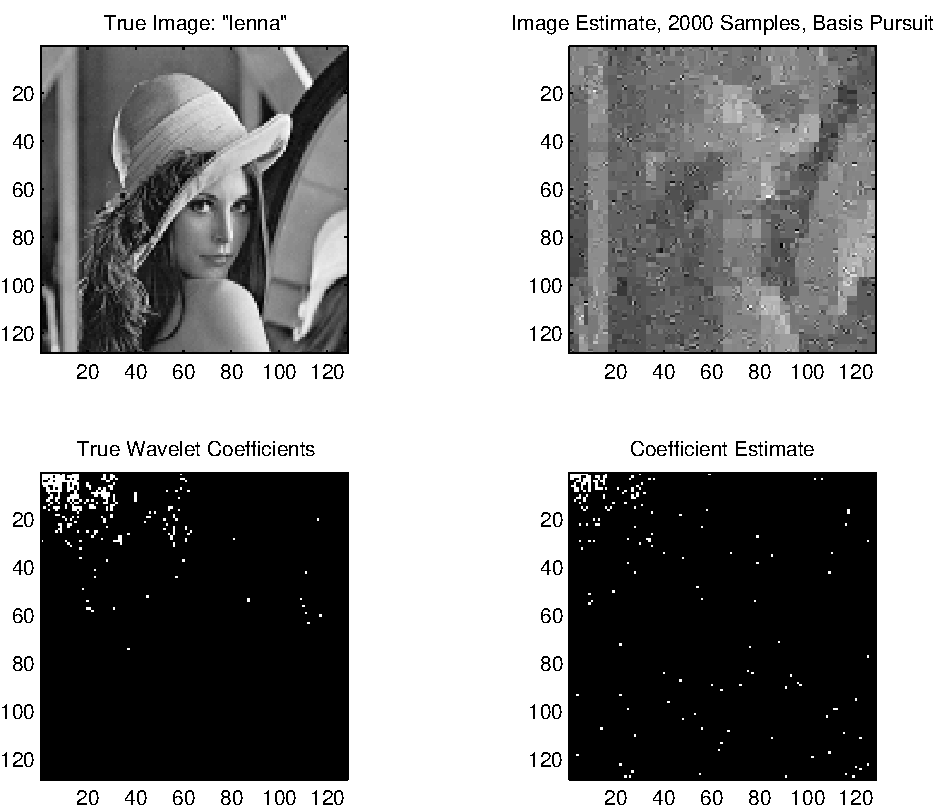
\includegraphics[width=0.4\textwidth]{lenna_m2000_cvx}%
  }%
  \qquad
  \subfloat[][]{%
    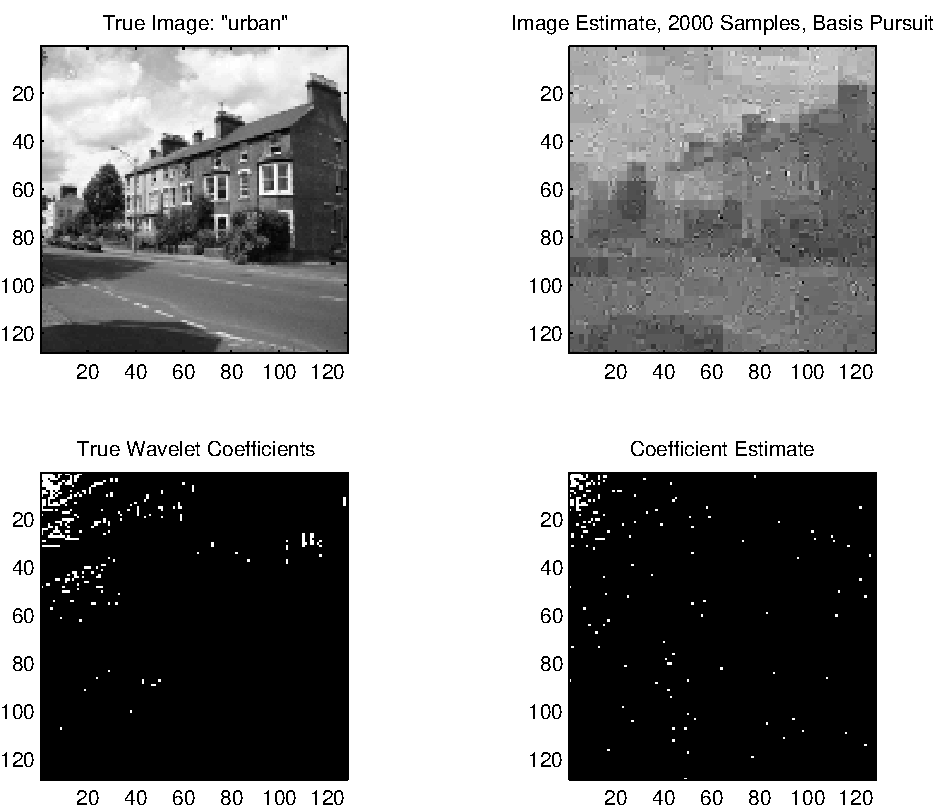
\includegraphics[width=0.4\textwidth]{urban_m2000_cvx}%
  } \\
  \subfloat[][]{%
    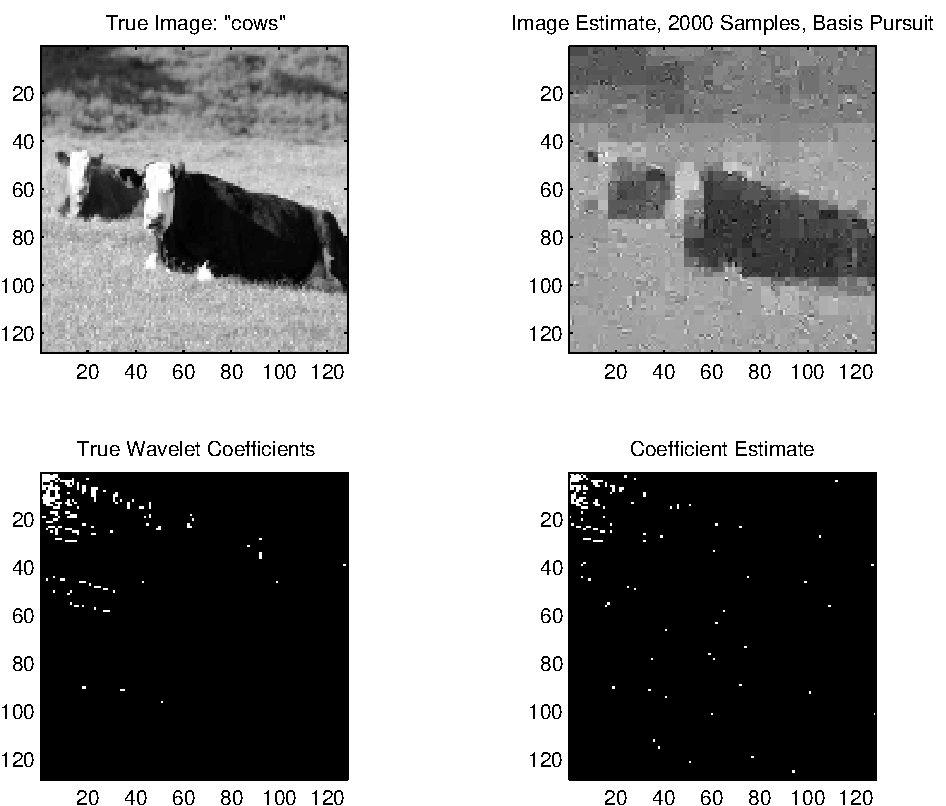
\includegraphics[width=0.4\textwidth]{cows_m2000_cvx}%
  }%
  \qquad
  \subfloat[][]{%
    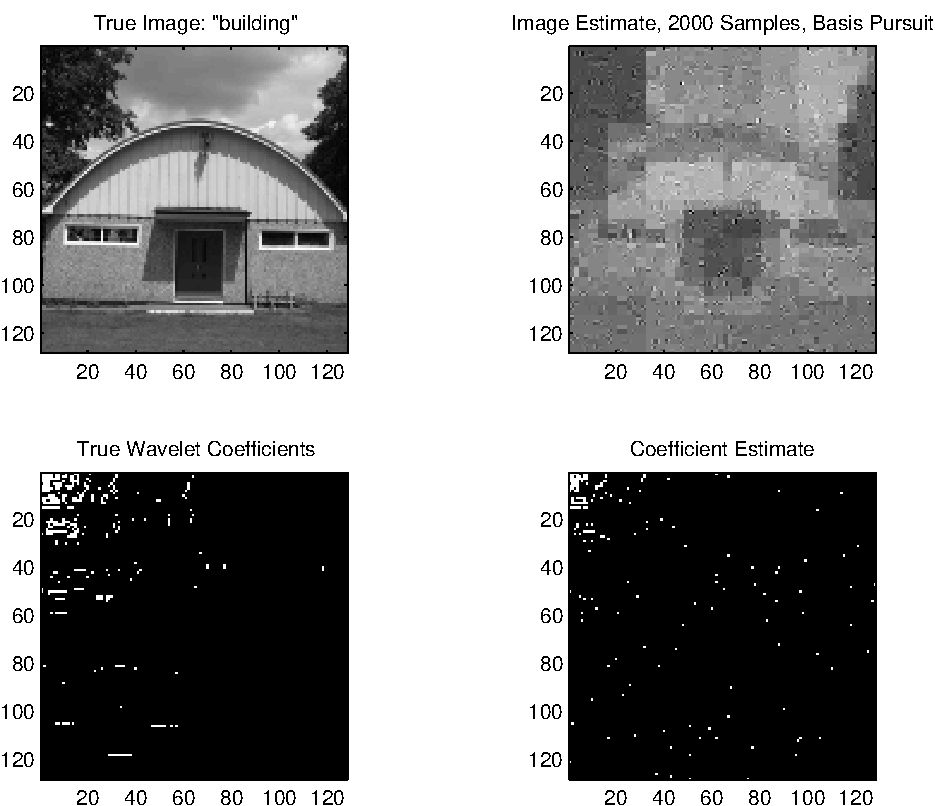
\includegraphics[width=0.4\textwidth]{building_m2000_cvx}%
  } \\
  \subfloat[][]{%
    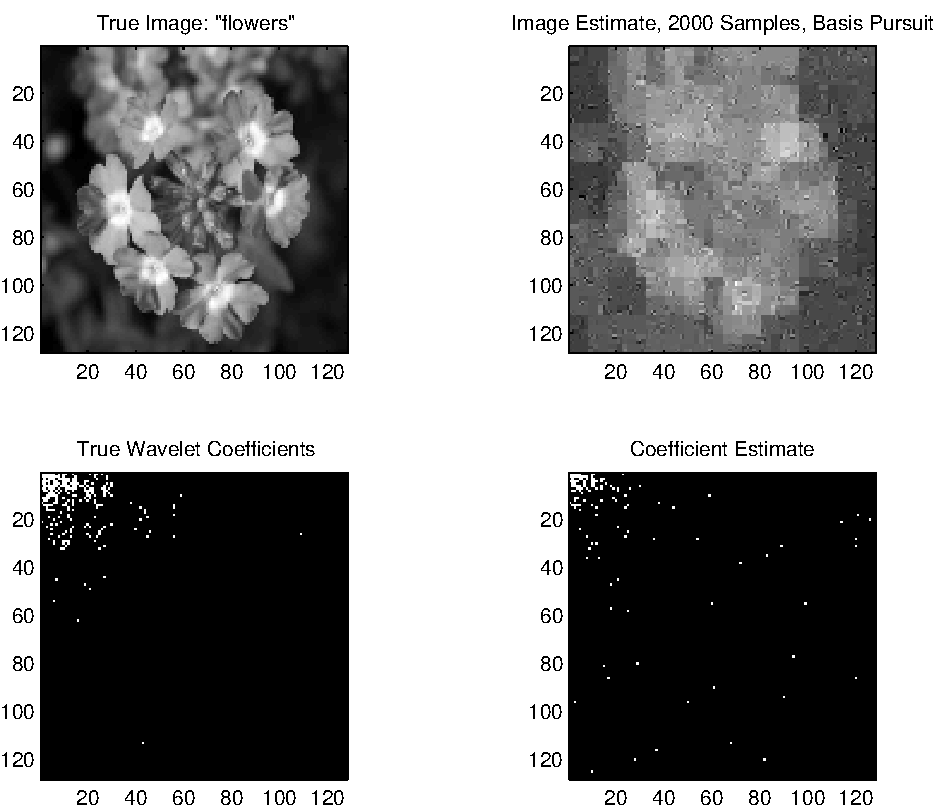
\includegraphics[width=0.4\textwidth]{flowers_m2000_cvx}%
  }%
  \qquad
  \subfloat[][]{%
    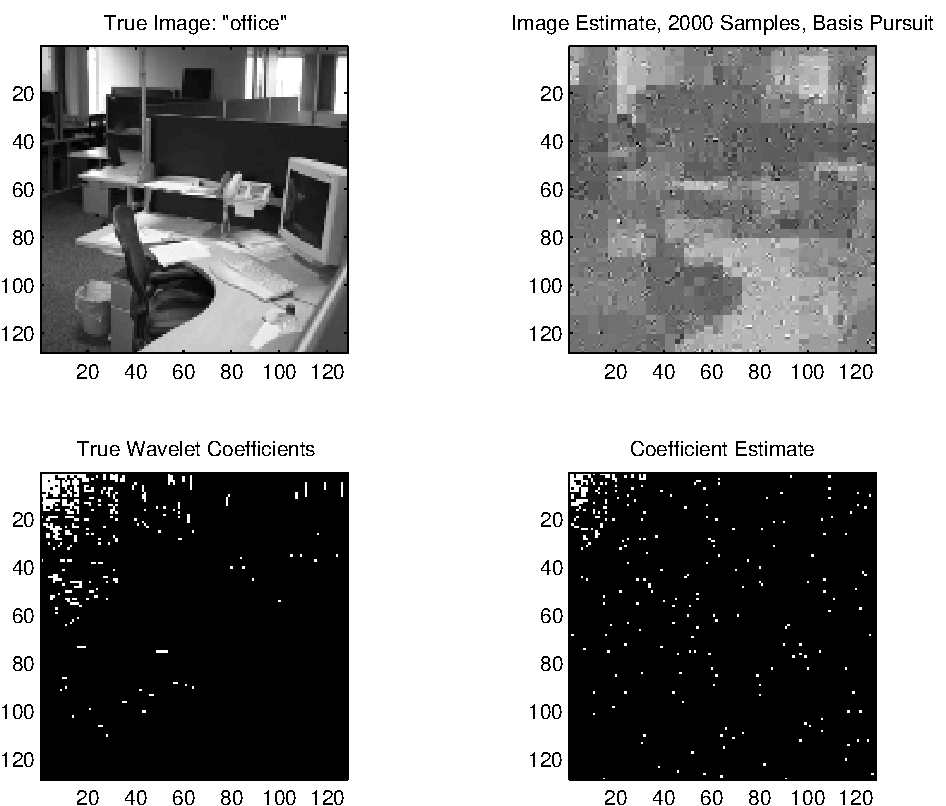
\includegraphics[width=0.4\textwidth]{office_m2000_cvx}%
  }
  \caption{Results of six trials of basis pursuit using 2000 data samples from a $128\times128$ image}
  \label{fig:bp-results}
\end{figure*}

\section{Conclusion}
We were not able to achieve the desired results using Bayesian methods.  As we began implementing the algorithm set forth in the paper, we realized how many parameters are involved.  Where the details are not explicit, we were forced to make educated guesses about important implementation decisions. This often led to unexpected results.  At times we were able to correct for such results, and other times it was unclear what was missing.

The nature of a probabilistic model is such that you set parameters to estimate a distribution. Since you do not know the exact values to give those parameters, you also estimate those, using more parameters.  This creates a hierarchy of hyperparameters which helps to fine-tune the estimation framework into a working state.  Unfortunately, we were unable to fine-tune our bayesian inference framework to where it made good estimates of the wavelet transform coefficients. We believe that once the model is appropriately tuned, it should be fairly robust to incoming data.

\bibliography{report}
\bibliographystyle{IEEEtran}

\end{document}


%%% Local Variables: 
%%% mode: latex
%%% TeX-master: t
%%% End: 



%  LocalWords:  compressive
